\section{Extremos de Funções de Várias Variáveis}

\begin{frame}[label=otimizacao]{Valores Extremos de Funções de duas Variáveis }
%\begin{scriptsize}

\uncover<1->{ \begin{defin} \begin{enumerate}
\item Dizemos que uma função $f$ de duas variáveis tem um \dt{valor máximo local} no ponto $(a,b)$ se existir  uma bola aberta $B_r(a,b)$ tal que $f(a,b)\geq f(x,y)$ para todo $(x,y)\in B_r(a,b)$.

\item Dizemos que uma função $f$ de duas variáveis tem um \dt{valor mínimo local} no ponto $(a,b)$ se existir  uma bola aberta $B_r(a,b)$ tal que $f(a,b)\leq f(x,y)$ para todo $(x,y)\in B_r(a,b)$.
\end{enumerate}
\end{defin}}

\begin{center}
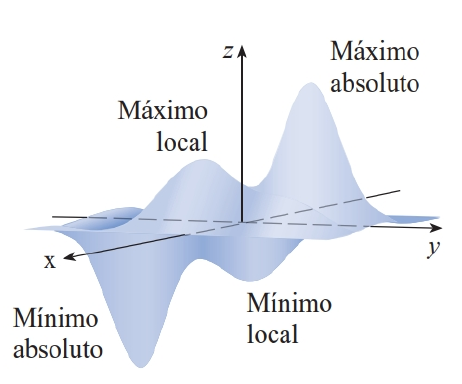
\includegraphics[scale=.4]{figuras/max-min1.png}
\end{center}

%\end{scriptsize}
\end{frame}


\begin{frame}[label=otimizacao]

\begin{teo} Se $f(x,y)$ tem um extremo local em $(a,b)$ e possui derivadas parciais em $(a,b)$, então 
\[\nabla f(a,b)=0.\]
\end{teo}

Um ponto $(a,b)$ tal que $\nabla f(a,b)$ não existe ou $\nabla f(a,b))=0$   é dito \dt{ ponto crítico ou ponto estacionário} de $f$.

\begin{minipage}{0.5\textwidth}
\begin{exe}
Determine os extremos relativos de $f(x,y)=x^2+y^2-2x-6y+14$
\end{exe}
\end{minipage}\ \
\begin{minipage}{0.3\textwidth}
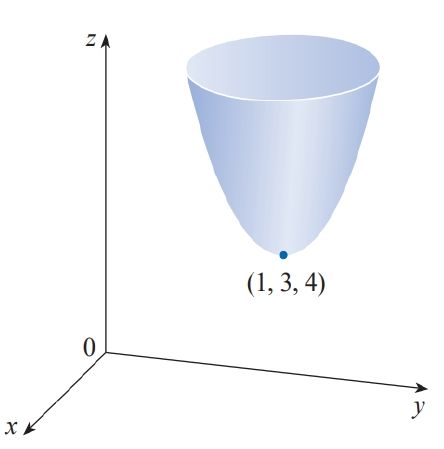
\includegraphics[scale=.4]{figuras/pnt-critico.png}
\end{minipage}

\end{frame}


\begin{frame}[label=otimizacao]
\begin{exe} A função $f(x,y)=y^2-x^2$ tem ponto crítico em $(0,0)$ mas não possui extremo relativo!
 \end{exe} 
 \begin{minipage}{0.5\textwidth}
 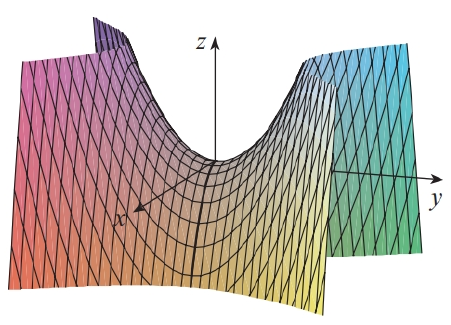
\includegraphics[scale=.5]{figuras/sela.png}
 \begin{center}
 
 ponto de sela
 \end{center}
 \end{minipage}
  \begin{minipage}{0.2\textwidth}
  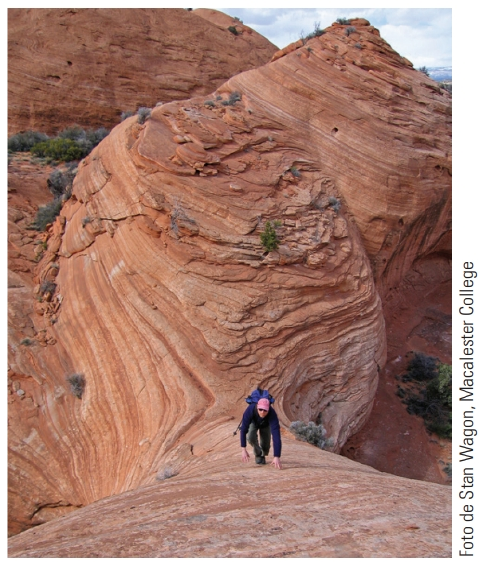
\includegraphics[scale=.4]{figuras/sela-montanha.png}
  \end{minipage}
\end{frame}


\subsection*{Matriz Hessiana}
\begin{frame}[label=otimizacao]
\frametitle{Matriz Hessiana }
%\begin{scriptsize}

Se $f$ é uma função de duas variáveis com todas as derivadas de ordem 2 no ponto $(a,b)$, definimos 
\[D^2f(a,b)=\left[\begin{array}{cc}
f_{xx}(a,b) & f_{xy}(a,b)\\
\\
f_{yx}(a,b) & f_{yy}(a,b)
\end{array}   \right],\]
chamada \dt{matriz Hessiana} da função $f$ no ponto $(a,b)$.



%\end{scriptsize}
\end{frame}

\subsection*{Teste da Segunda Derivada}
\begin{frame}[label=otimizacao]
\frametitle{Teste da Segunda Derivada}

\begin{teo}[Teste da Segunda Derivada]

Seja $z=f(x,y)$ uma função de classe $C^2$ em uma bola $B_r(a,b)$ tal que $\nabla f(a,b)=(0,0)$. Neste caso,
\begin{enumerate}[a]
\item Se $\det D^2f(a,b)>0$ e $f_{xx}(a,b)<0$, então $(a,b)$ é máximo local.

\item Se $\det D^2f(a,b)>0$ e $f_{xx}(a,b)>0$, então $(a,b)$ é mínimo local.

\item Se $\det D^2f(a,b)<0$, então $(a,b)$ é ponto de sela.


\end{enumerate}
\end{teo}

\begin{obs}
Se $\det D^2f(a,b)=0$, nada podemos concluir.
\end{obs}

%%\begin{exe} \begin{enumerate}
%%\item Localize e classifique os pontos críticos de $f(x,y)=2x^3+y^3-3x^2-3y$.
%%
%%\item O gráfico da função $g(x,y)=\frac{1}{xy}$ é uma superfície $S$ em $\R^3$. Encontre os pontos de $S$ mais próximos da origem.
%%\end{enumerate}
%\end{exe}



\end{frame}

\begin{frame}[label=otimizacao]
\begin{exe}
Localize e classifique os pontos críticos de $f(x,y)=x^4+y^4-4xy+1$.
\end{exe}
 \begin{minipage}{0.5\textwidth}
 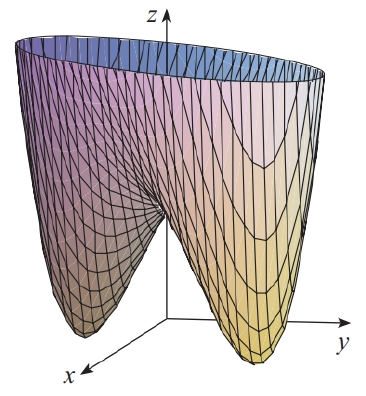
\includegraphics[scale=.5]{figuras/teste-derv2.png}
 \begin{center}
 \end{center}
 \end{minipage}
  \begin{minipage}{0.2\textwidth}
  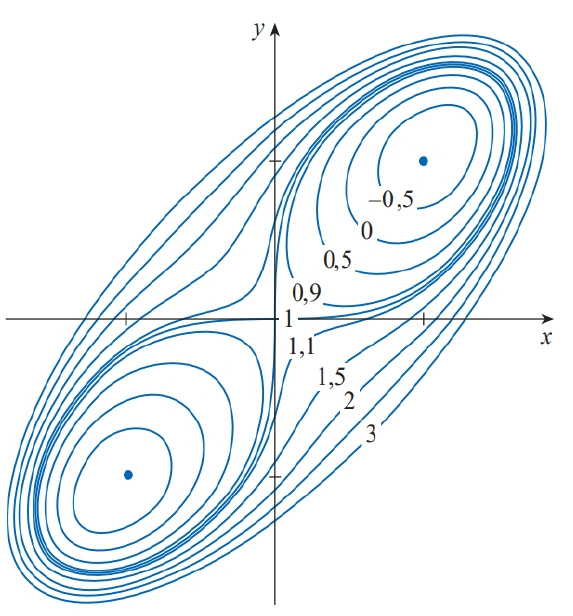
\includegraphics[scale=.4]{figuras/mapa-cont.png}
  \end{minipage}
\end{frame}

\begin{frame}[label=otimizacao]
\begin{casa}
Uma caixa retangular  sem tampa deve ser feita com 12 m$^2$ de papelão. Determine o volume máximo da caixa.
\end{casa}
\end{frame}


\subsection*{Máximos e Mínimos Absolutos}
\begin{frame}[label=otimizacao]
\frametitle{ }


\uncover<1->{\begin{defin}
Seja uma função $f$ de duas variáveis definida em um conjunto $U\subset \R^2$.
\begin{enumerate}


\item Dizemos que $f$  tem um valor \dt{máximo absoluto} em $U$ se existir um ponto $(a,b)\in U$ tal que $f(a,b)\geq f(x,y)$ para todo $(x,y)\in U$. Neste caso, $f(a,b)$ é {\color{red} o valor máximo absoluto }de $f$ em $U$. 

\item Dizemos que $f$  tem valor \dt{mínimo absoluto} em $U$ se existir um ponto $(a,b)\in U$ tal que $f(a,b)\leq f(x,y)$ para todo $(x,y)\in U$. Neste caso, $f(a,b)$ é {\color{red}o valor mínimo absoluto} de $f$ em $U$
\end{enumerate} 
\end{defin} 

\begin{exe} \begin{enumerate}
\item A função  $f(x,y)=1-x^2-y^2$ tem máximo absoluto em $\R^2$ no ponto $(0,0)$.

\item A função $f(x,y)=x$ não tem máximo nem mínimo absoluto em $\R^2$.
\end{enumerate} 
\end{exe}}



\end{frame}
\subsection*{Topologia no plano}
\begin{frame}[label=otimizacao]{Topologia no plano}
Antes de enunciarmos nosso próximo resultado, precisamos de algumas noções topológicas no plano.


\begin{minipage}{0.7\textwidth}
\begin{itemize}
\item Um conjunto é dito {\color{orange}limitado} se ele está contido em algum disco.

\item A \dt{fronteira} de um conjunto $D$, denotada por $\partial D$, é formada por pontos $(a,b)$ tais que qualquer disco aberto com centro em $(a,b)$ contém pontos de $D$ e pontos que não estão em $D$.


\item Um conjunto $D$ de $\R^2$ é dito \dt{fechado} se contém todos os pontos de sua fronteira, onde 

\item Um conjunto \dt{fechado} e {\color{orange}limitado} é dito ser \dt{compacto}.

\item Um conjunto  é {\color{red} aberto} quando seu complementar é fechado.


\end{itemize}

\end{minipage}
\begin{minipage}{0.2\textwidth}
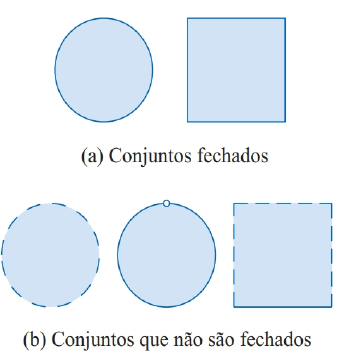
\includegraphics[scale=.4]{figuras/fechados.png}
\end{minipage}



\end{frame}


\subsection*{Teorema de Weierstrass}
\begin{frame}[label=otimizacao]
\uncover<1->{\begin{teo}[Teorema de Weierstrass]
Se $f$ é uma {\color{red}função contínua} definida em um {\color{red}conjunto fechado e limitado} $D$ então $f$ {\color{blue}assume valor máximo e mínimo absolutos} em $U$.
\end{teo}}

\begin{exampleblock}{Determinação de Extremos Absolutos}
Para determinarmos os extremos absolutos de uma {\color{red}função contínua} definida em um {\color{red}conjunto fechado e limitado} $D$:
\begin{enumerate}
\item Determinar os valores de $f$ nos pontos críticos de $f$ em $D$.
\item Determinar os valores extremos de $f$ na fronteira de $D$.
\item O maior dos valores dos passos anteriores será o máximo absoluto e o menor deles o valor mínimo absoluto.
\end{enumerate}
\end{exampleblock}
\end{frame}

\begin{frame}[label=otimizacao]
\begin{exe}
Determine os valores extremos da função $f(x,y)=x^2-2xy+2y$ no retângulo $D=\{(x,y) |\ 0\leq x\leq 3, 0\leq y\leq 2 \}$.
\end{exe}

\begin{minipage}{0.45\textwidth}
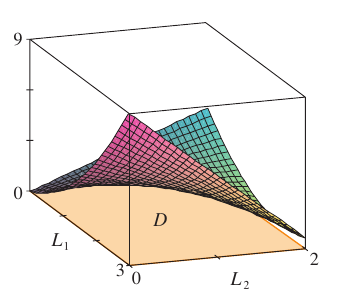
\includegraphics[scale=0.5]{figuras/sec-15_7-fig13.png}
\end{minipage}
\begin{minipage}{0.45\textwidth}
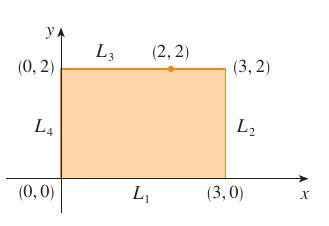
\includegraphics[scale=0.5]{figuras/max1.png}
\end{minipage}
\end{frame}



%\begin{frame}
%\frametitle{ }
%\begin{scriptsize}
%
%\uncover<1->{\begin{exe}\begin{enumerate}
%\item Econtre o máximo e o mínimo da função $f(x,y)=(x-2)^2y+y^2-y$ definida em $D=\{(x,y)\in \R^2;\ x\geq 0, y\geq 0 \mbox{ e } x+y\leq 4\}$
%
%\item Uma placa metálica circular com um metro de raio está colocada com centro na origem do plano $xy$ e é aquecida de modo que a temperatura num ponto $(x,y)$ é dada por
%$$T(x,y)=64(3x^2-2xy+3y^2+2y+5),$$
%graus Celcius, onde $x,y$ estão em metros. Encontre a maior e a menor temperatura na placa.
%
%\end{enumerate} 
%\end{exe} }
%
%\end{scriptsize}
%\end{frame}




\subsection*{Multiplicadores de Lagrange}
\begin{frame}[label=otimizacao]
\frametitle{Multiplicadores de Lagrange  em duas Variáveis}


\begin{teo}Sejam $f(x,y)$ e $g(x,y)$ funções de classe $C^1$ definidas em um aberto $U$ que contém a curva $C$ de equação $g(x,y)=k$. Se $f(x,y)$ restrita à curva $C$ assume um valor máximo ou mínimo em $(x_0,y_0)\in C$ e {\color{red}$\nabla g(x_0,y_0)\neq \vec{0}$}, então existe {\color{blue}$\lambda\in \R$ }tal que
\[\nabla f(x_0,y_0)={\color{blue}\lambda} \nabla g(x_0,y_0)\]
\end{teo} 

\begin{center}
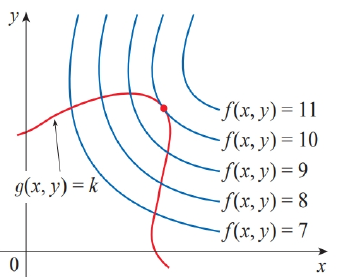
\includegraphics[scale=.5]{figuras/sec14_8-fig1.png}
\end{center}


\end{frame}


\begin{frame}[label=otimizacao]
\begin{exe}
Determine os valores extremos da função $f(x,y)=xy$ no círculo $x^2+y^2=1$.
\end{exe}

\begin{minipage}{0.55\textwidth}
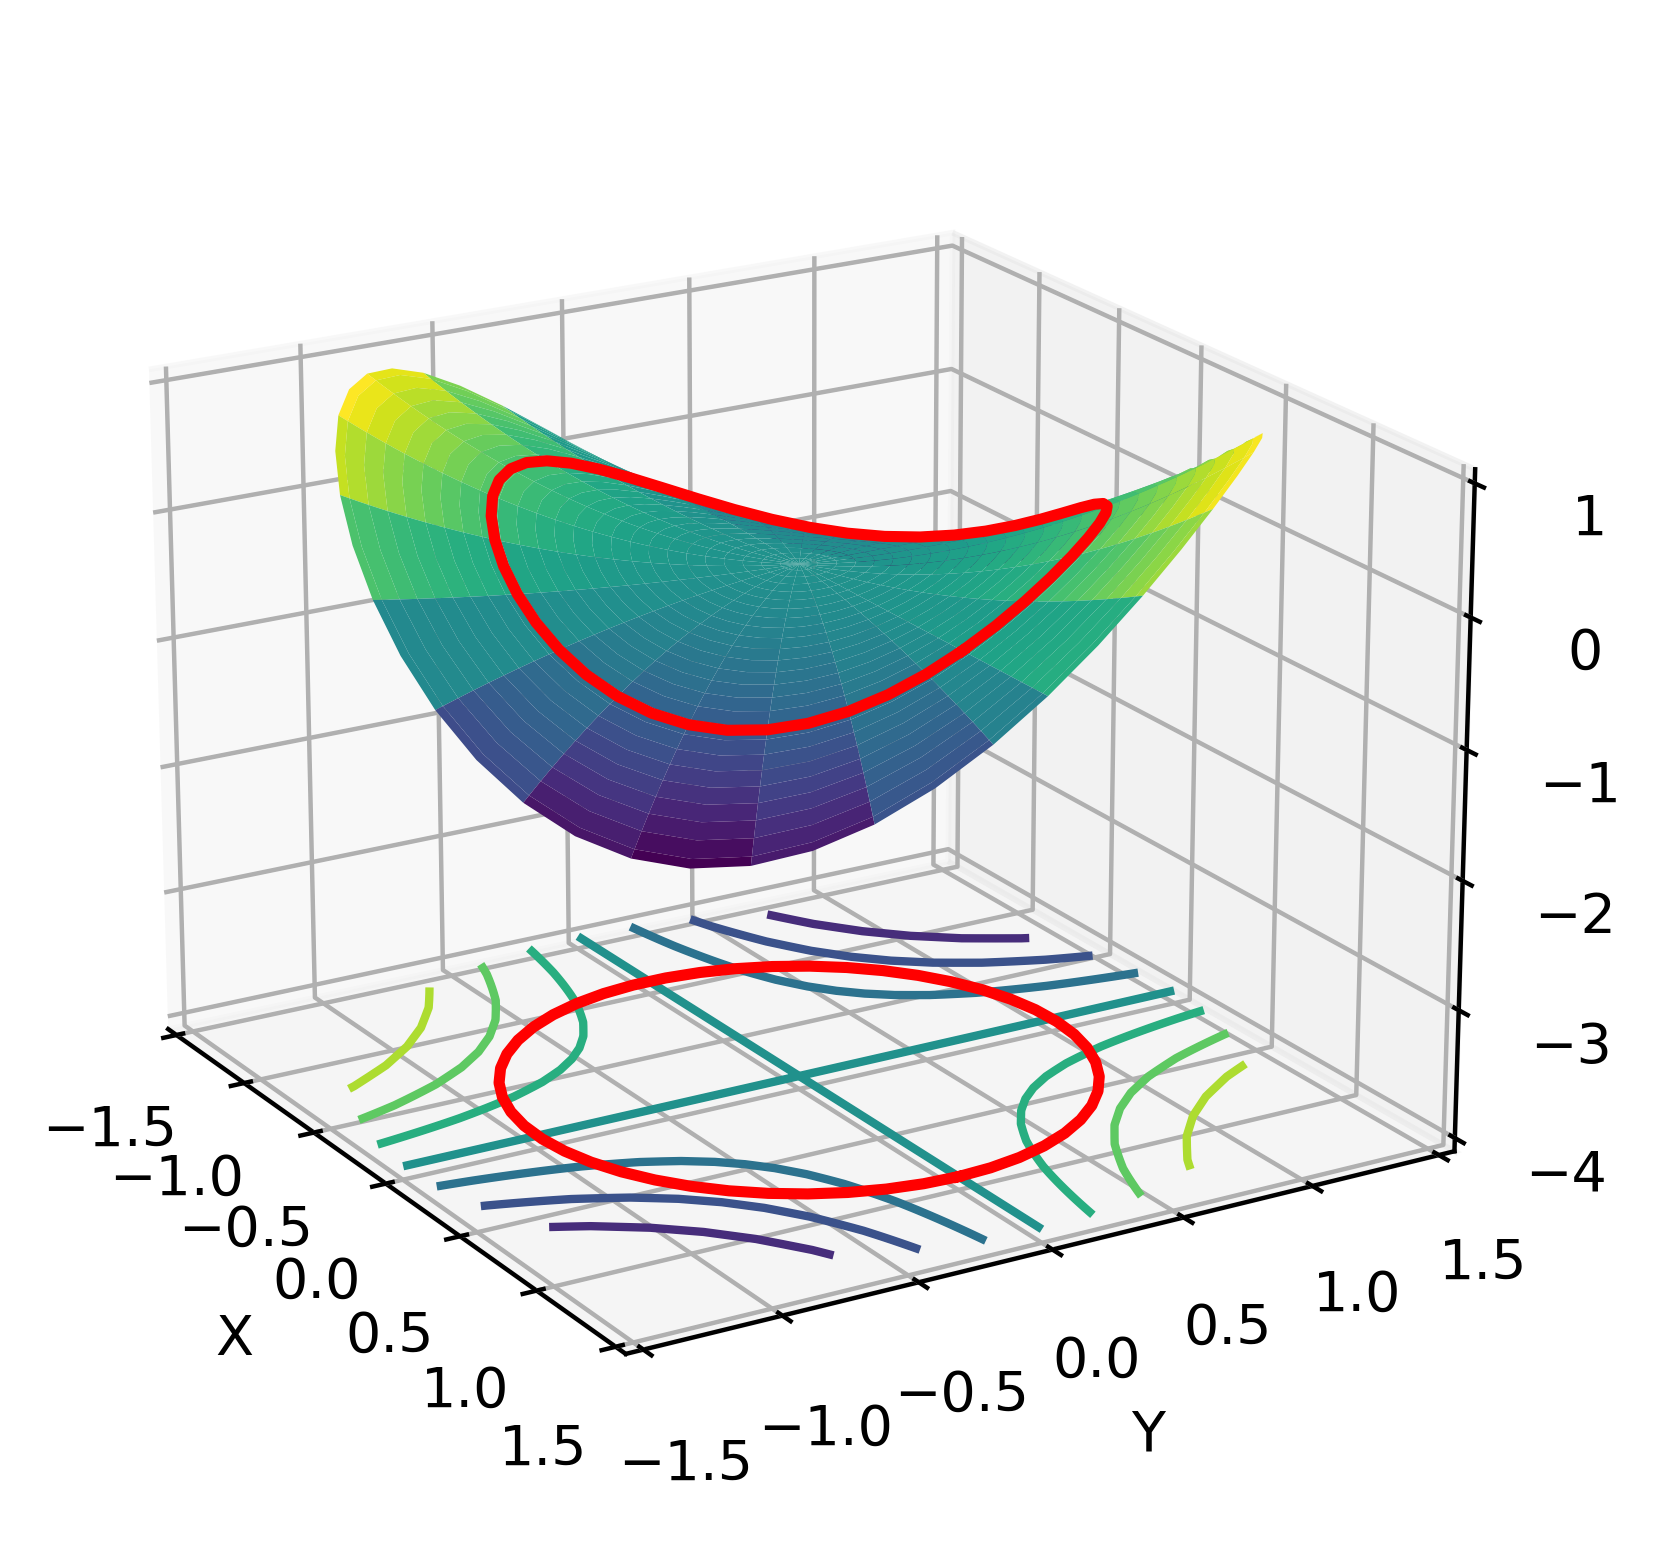
\includegraphics[scale=.6]{figuras/exemplo-lagrange1.png}
\end{minipage}
\begin{minipage}{0.4\textwidth}
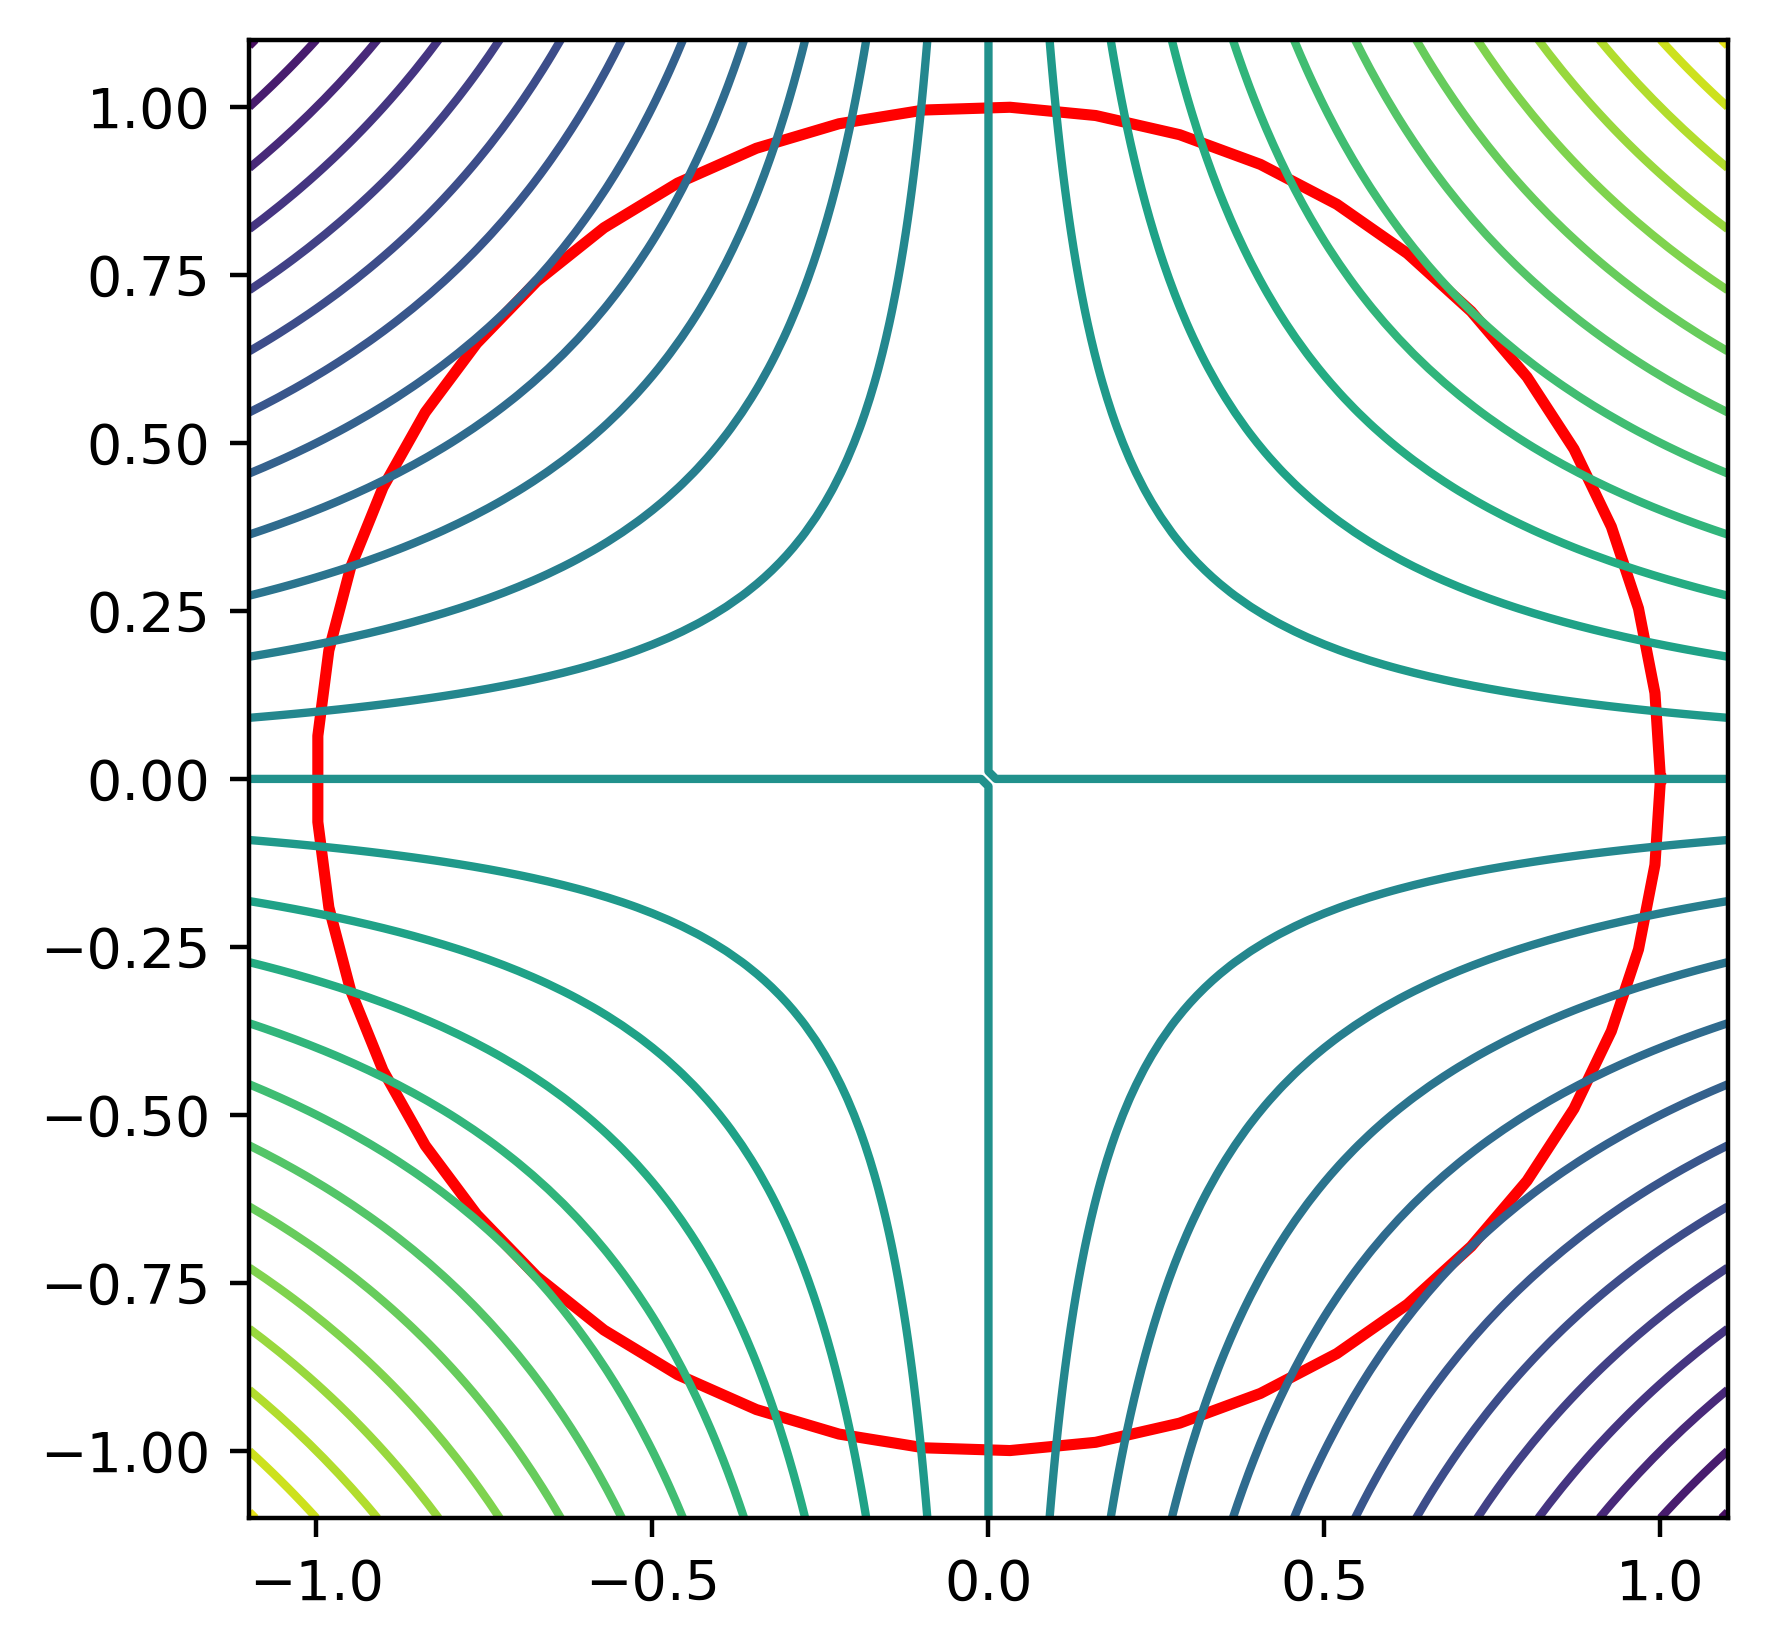
\includegraphics[scale=.45]{figuras/exemplo-lagrange-curvas-nivel.png}
\end{minipage}
\end{frame}

\begin{frame}[label=otimizacao]
\begin{casa}
Determine os pontos da hipérbole $x^2+8xy+7y^2-225=0$ que estão mais próximos da origem.
\end{casa}
\end{frame}

%\begin{exe}
%\begin{exe} \begin{enumerate}
%\item Determine os pontos extremos de $f(x,y)=xy$ tais que $x^2+y^2=1.$
%
%\item Determine os pontos extremos de $f(x,y)=x^2+2y^2$ tais que $x^2+y^2\leq 1.$
%
%
%\end{enumerate}
%\end{exe}
%\end{exe}


\begin{frame}[label=otimizacao]
\frametitle{ }
%\begin{scriptsize}
\begin{teo}Sejam $f(x,y,z)$ e $g(x,y,z)$ funções de classe $C^1$ definidas em um aberto $U$ que contém a superfície $S$ de equação $g(x,y,z)=k$. Se $f(x,y,z)$ restrita à superfície $S$ assume um valor máximo ou mínimo em $P_0=(x_0,y_0,z_0)\in S$ e $\nabla g(x_0,y_0,z_0)$ não é nulo, então existe $\lambda\in \R$ tal que
\[\nabla f(x_0,y_0,z_0)=\lambda \nabla g(x_0,y_0,z_0)\]
\end{teo} 

\begin{exe}
Determine os pontos da esfera $x^2+y^2+z^2=4$ que estão mais próximos e mais distantes do ponto $(3,1,-1)$.
\end{exe}

%\begin{exe} Encontre as dimensões da caixa retangular de maior volume que pode ser inscrita no elipsóide de equação $\dps \frac{x^2}{9}+\frac{y^2}{4}+z^2=1$, cujas arestas são paralelas aos eixos coordenados.
%\end{exe}}

%\end{scriptsize}
\end{frame}

\begin{frame}[label=otimizacao]
\frametitle{Multiplicadores de Lagrange com Duas Restrições}

\begin{teo}Sejam $f(x,y,z)$, $g_1(x,y,z)$ e $g_2(x,y,z)$  funções de classe $C^1$ definidas em um aberto $U$ que contém a curva $C$ de interseção das superfícies de equações $g_1(x,y,z)=k_1$ e $g_2(x,y,z)=k_2$. Se $f(x,y,z)$ restrita à curva  $C$ assume um valor máximo ou mínimo em $P_0=(x_0,y_0,z_0)\in S$ e $\nabla g_1(x_0,y_0,z_0)\times \nabla g_2(x_0,y_0,z_0)$ não é nulo, então existem $\lambda, \mu \in \R$ tais que
$$\nabla f(x_0,y_0,z_0)=\lambda \nabla g_1(x_0,y_0,z_0)+\mu \nabla g_1(x_0,y_0,z_0)$$ \end{teo} 

%\begin{exe} Encontre os pontos de máximo e mínimo de $f(x,y,z)=x+y+z$ sujeito às restrições $x^2+y^2=2$ e $x+z=1$.
%\end{exe}


\end{frame}


\begin{frame}[label=otimizacao]
\begin{exe}
Determine o valor máximo da função $f(x,y,z)=x+2y+3z$ na curva da interseção do plano $x-y+z=1$ com o cilindro $x^2+y^2=1$.
\end{exe}
\begin{center}
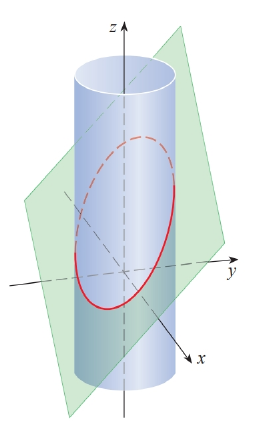
\includegraphics[scale=0.6]{figuras/sec14_8-fig8.png}
\end{center}
\end{frame}